%Author: Siddhesh Wani
%Date: December 22, 2015




\documentclass[12pt]{article}
\usepackage{tikz}
\usetikzlibrary{shapes.geometric, arrows}
\usepackage{hyperref}
\usepackage[a4paper]{geometry}
\usepackage[font=small]{caption}


%DO NOT EDIT start
%Define different shapes to be used in flowchart
\tikzstyle{startstop} = [rectangle, rounded corners, minimum width=3cm, minimum height=1cm,text centered, draw=black, fill=red!30]
\tikzstyle{io} = [trapezium, trapezium left angle=70, trapezium right angle=110, minimum width=3cm, minimum height=1cm, text centered, draw=black, fill=blue!30]
\tikzstyle{process} = [rectangle, minimum width=3cm, minimum height=1cm, text centered, draw=black, fill=orange!30]
\tikzstyle{decision} = [diamond, minimum width=3cm, minimum height=1cm, text centered, draw=black, fill=green!30]
\tikzstyle{arrow} = [thick,->,>=stealth]
\tikzstyle{connector} = [signal,draw=black,fill=olive!30]%,text width=1cm,text height=1.5cm,align=center]
%DO NOT EDIT end


\begin{document}



\section{User manual for Scilab2C}



% 
% This flow chart describes steps to be followed for using `scilab2c' extenstion.
% 
% \begin{tikzpicture}[node distance=2cm]
% \label{first}
% 
% \node (start) [startstop] {Start};
% \node (open$_$gui)[process, text width=7cm,  below of=start] {Open scilab2c gui in Scilab by typing `sci2c\_gui' in command window};
% \node (no$_$of$_$files) [decision, below of=open$_$gui, text width=2cm, yshift=-1.5cm] {Does scilab code consists of multiple files?};
% \node (single$_$file) [process, below of=no$_$of$_$files, text width=5cm, yshift=-1cm, xshift=-4cm] {Select scilab file by clicking 'Browse' against 'Main file name'};
% \node (multi$_$files) [process, below of=no$_$of$_$files, text width=5cm, yshift=-1cm, xshift= 4cm] {Select main scilab file by clicking 'Browse' against 'Main file name'};
% \node (sub$_$functions) [process, below of=multi$_$files,text width=6cm]{Select \textbf{folder} containing other scilab functions by clicking 'Browse' against 'Sub-functions'};
% \node (out$_$dir) [process, below of=no$_$of$_$files, text width=5cm, yshift=-5cm] {Select folder in which to store results of conversion};
% \node (run$_$mode) [process, below of=out$_$dir] {Select 'All' for 'Run mode'};
% \node (A) [connector,below of=run$_$mode, signal to=south] {A};
% 
% \draw [arrow] (start) -- (open$_$gui);
% \draw [arrow] (open$_$gui) -- (no$_$of$_$files);
% \draw [arrow] (no$_$of$_$files) -| node[anchor=east] {yes} (multi$_$files);
% \draw [arrow] (no$_$of$_$files) -| node[anchor=west] {no} (single$_$file);
% \draw [arrow] (multi$_$files) -- (sub$_$functions);
% \draw [arrow] (single$_$file) |- (out$_$dir); 
% \draw [arrow] (sub$_$functions) |- (out$_$dir);
% \draw [arrow] (out$_$dir) -- (run$_$mode);
% \draw [arrow] (run$_$mode) -- (A);
% \end{tikzpicture}
% 
% 
% \begin{tikzpicture}[node distance=2cm]
% \node (A) [connector, signal to=north] {A};
% \node (target) [process, below of=A] {Select required 'Target'};
% \node (copy$_$code) [process, below of=target] {Select desired choice for `Copy scilab code into C'};
% \node (tool) [process, below of=copy$_$code] {Select desired choice for `Tool to compile generated C code'};
% \node (convert) [process, below of=tool] {Press `Convert' to start the conversion};
% \node (stop) [startstop, below of=out$_$dir] {Stop};
% 
% \draw [arrow] (A) -- (target); 
% \draw [arrow] (target) -- (copy$_$code);
% \draw [arrow] (copy$_$code) -- (tool);
% \draw [arrow] (tool) -- (convert);
% \draw [arrow] (convert) -- (stop);
% 
% 
% \end{tikzpicture}

This section describes steps to be followed for using Scilab2C. Pre-requisites are mentioned followed by procedure to install Scilab2C.
\\

\subsection{Installation}
\subsubsection{Prerequisites}
There are few prerequisites or some packages must be pre installed before we can use Scilab2C. These are:
\begin{itemize}
  \item scilab $>$=5.5.1.
  \item scilab-arduino toolbox (If using Scilab2C to generate code for Arduino)
  \item Arduino makefile (https://github.com/sudar/Arduino-Makefile). Install using `sudo apt-get install arduino-mk’.
  \item BCM2835 C library for RasberryPi (http://wiringpi.com/)
  \item RasberryPi tools (For cross compiling code for RasberryPi)
\end{itemize}

\subsubsection{Installing Scilab2C}
Before we can use `Scilab2C' extension, we need to install latest version of Scilab2C. Follow following procedure to get latest source code from github repo.
\begin{itemize}
  \item Open terminal window. (Ctrl+Shift+T is shortcut).
  \item Change current directory to `/path/to/scilab/share/scilab/contrib'
  \item Clone the git repo using following command:\\ 
\indent\indent\texttt{git clone https://github.com/siddhu8990/Scilab2C.git}
  \item Make sure a directory named `Scilab2C' is present in `contrib' folder.
  \item Open Scilab.
  \item Run `builder.sce’ file present in ‘Scilab2C/2.3-1’ using 'exec'. This generates binary files from source files.\\
  \indent\indent\texttt{exec(“/path/to/Scilab2C/2.3-1/builder.sce”)}
  \item In `Home/.scilab/scilabx.x.x' make a new file `.scilab' if it does not exist already. Open ‘.scilab’ using suitable editor. Add following line in this file:\\
  \indent\indent\texttt{exec(“/path/to/Scilab2C/2.3-1/loader.sce”)}\\
This will load the `scilab2c' everytime scilab is started.

\end{itemize}

\subsubsection{Installing supporting packages}
Most of the supporting packages or libraries which are required are provided with the toolbox. But they were compiled using
latest source code available at release of toolbox. If you want to use latest libraries, steps to compile the same are listed 
below. You can follow these steps and replace old files with newly generated ones.
\begin{itemize}
 \item scilab-arduino toolbox
  
 %\end{itemize}
  \hypertarget{tools}{}
  \item{\textbf{RasberryPi tools}}
    \begin{itemize}
   \item Make a folder named `RasberryPi tools' somewhere on the harddisk. 
   \item Open terminal and change directory to `RasberryPi tools'. Clone `Tools' repo using `git clone https://github.com/raspberrypi/tools.git'.
   \item Add location of toolchain to your `PATH' variable.\\ \texttt{`export PATH=\$PATH:/location/of/tools/folder/arm-bcm2708/gcc-linaro-arm-linux-gnueabihf-raspbian/bin'} 
  \end{itemize}

   \item{\textbf{ BCM2835 C library for RasberryPi}}
   \begin{itemize}
   \item Before going further, make sure that you have installed `RasberryPi tool' following 
   the instructions given above.
   \item Download latest source code from `\url{http://www.airspayce.com/mikem/bcm2835}'.
   \item Extract source code at some suitable location on harddrive.
   \item Open the terminal window and change current directory to the location where 
   source is extracted.
   \item Execute following command \\
   \texttt{./configure -host=arm CC=arm-linux-gnueabihf-gcc ar=arm-linux-gnueabihf-ar}
   \item Then execute `make' to cross compile the library. Don't do `make install' as it is noramlly next step. 
   \end{itemize}
   
   \item{\textbf{ Cross compiling Lapack and Blas for RasberryPi}}
   \begin{itemize}
    \item Download latest source code for Lapack from `\url{http://www.netlib.org/lapack/}'. Extract source files at some suitable location.
    \item Open file `make.inc.example' given in Lapack folder using some editor.
    \item Edit following items as shown:
    \begin{itemize}
     \item FORTRAN = arm-linux-gnueabihf-gfortran
     \item LOADER = arm-linux-gnueabihf-gfortran
     \item CC = arm-linux-gnueabihf-gcc
     \item ARCH = arm-linux-gnueabihf-ar
     \item RANLIB = arm-linux-gnueabihf-ranlib
    \end{itemize}
    \item Since we are cross compiling for some other platform, normal way compiling 
    will not work.
    \item Open terminal window and change current directory to laplack directory.
    \item We will need to compile BLAS, CBLAS and Lapack separately and in same order.
    \item Change current directory to /path/to/lapack/BLAS/SRC and run `make'. This will generate `librefblas.a' in Lapack folder.
    \item Now change current directory to /path/to/laplack/CBLAS and run `make'. This will generate `libcblas.a' in Lapack folder.
    \item Now change current directory to /path/to/laplack/SRC and run `make'. This will generate `liblapack.a' in Lapack folder.
    Now replace the generated lib files in 'src/c/hardware/rasberrypi/libraries' in `scilab2c' source folder.
   \end{itemize}
   
   \item{\textbf{ GNU Scientific Library (GSL) for RasberryPi}}
   \begin{itemize}
   \item Before going further, make sure that you have installed `RasberryPi tool' following 
   the instructions given \hyperlink{tools}{here}.
   \item Get latest source code for GSL from \url{ftp://ftp.gnu.org/gnu/gsl/}.
   \item Extract source code at some suitable location on harddrive.
   \item Open the terminal window and change current directory to the location where 
   source is extracted.
   \item Execute following command \\
   \texttt{./configure -host=arm CC=arm-linux-gnueabihf-gcc ar=arm-linux-gnueabihf-ar --enable-static}
   \item Then execute `make libgsl.la' to cross compile the library. Don't do `make install' as it is noramlly next step.
   \item Library `libgsl.a' is created in folder `.libs'. By default this folder is hidden.
   \item Now replace the generated lib file in 'src/c/hardware/rasberrypi/libraries' in `scilab2c' source folder.
   
   
   \end{itemize}
   
\end{itemize}

\subsection{Using Scilab2C for C code generation}
Scilab2C extension in scilab can be used for generating C code from a scilab script. Currently it supports three types of target platforms:
\begin{itemize}
 \item \textbf{Standalone C code}: General C code which can be compiled using any compiler.
 \item \textbf{Arduino} : Generated code with few additions can be run on an Arduino board. (A scilab-arduino extension is required)
 \item \textbf{AVR} : Code can be generated for using hardware peripherals of AVR microcontroller

\end{itemize}


You can follow following steps for generating C code using scilab2c extension for required target platforms.
\begin{itemize}
 \item \textbf{Generating standalone C code}
 \begin{enumerate}
  \item Write the scilab script first which is to be converted to C. Scilab code can contain single file or many files, but each file must be a scilab function. 
  There must be one main scilab file in case project contains many files, from which execution of code starts. All scilab files must be in a single folder. 
  
  \begin{figure}[h]
  {
  \centering
   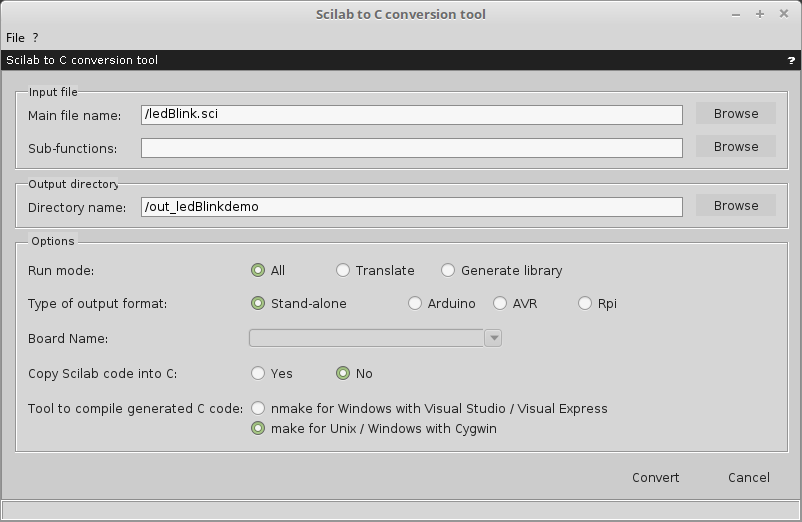
\includegraphics[scale=0.4]{img/sci2cgui}
   \caption{\small{GUI for `Scilab2C'}}
   \label{fig:gui}
  }
  \end{figure}
  
  
  \item Type `sci2c\_gui' or `scilab2c' in scilab console. This will prompt the GUI of Scilab2C extension as shown in figure  \ref{fig:gui}
  
  \begin{figure}
  
  {
  \centering 
   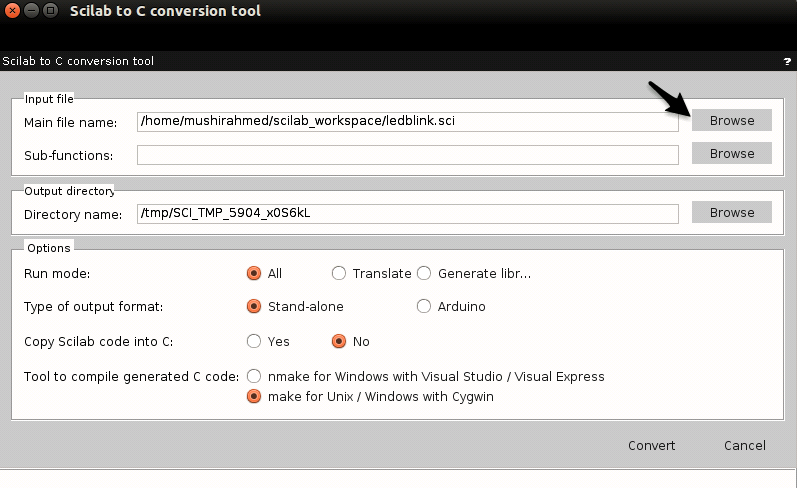
\includegraphics[scale=0.4]{img/gui_pick_file}
   \caption{\small{Select `main' scilab file for conversion}}
   \label{fig:main}
  }
  \end{figure}
  

  \item Click `Browse' next to `Main file name' textbox, browse to location of main scilab file and select it. (Refer figure \ref{fig:main})
  \item If scilab code contains many files, select folder containing these file by clicking `Browse' next to `Sub-functions' textbox.
  \begin{figure}
  \centering
  {
   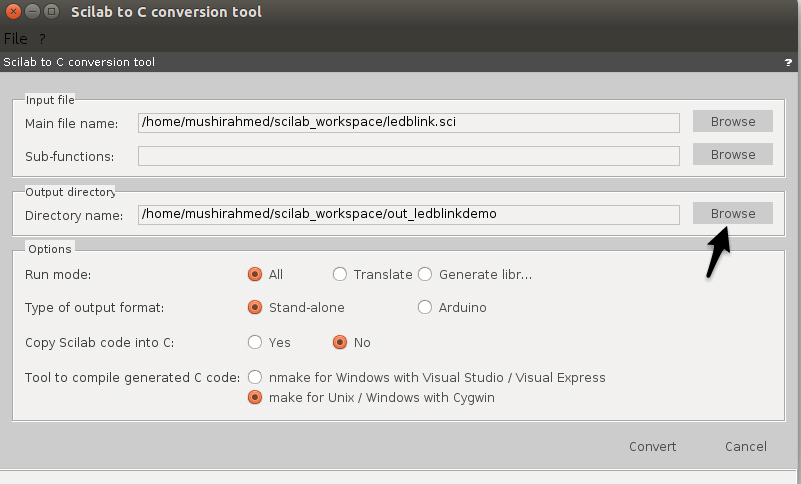
\includegraphics[scale=0.4]{img/gui_out_pickup}
   \caption {\small{Select output folder}}
   \label{fig:output}
  }
  \end{figure}

  \item Create a new folder somewhere on the disk, preferably in same folder containing scilab files. Select this newly created folder by clicking 
  `Browse' next to `Directory name' textbox. (Refer figure \ref{fig:output})
  \item Choose appropriate options from `Options' box. Different options are explained below:
  \begin{enumerate}
   \item Run mode : If only directory structure is to generated in output directory, select `Generate library'. If only conversion of scilab files is to be done, select
   `Translate'. In case both are to be done, select `All'. 
   \item Target platform : To generate standalone C code, select `Standalone C' from dropdown. (Refer figure \ref{fig:standalone})
  \begin{figure}
  \centering
  {
   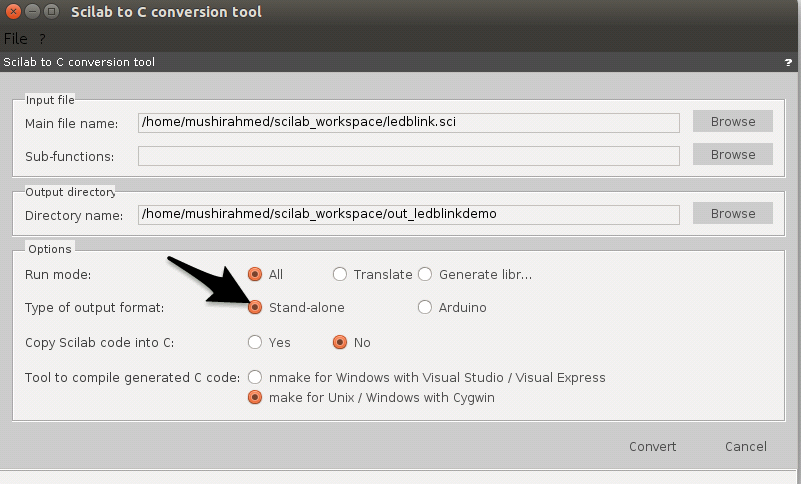
\includegraphics[scale=0.4]{img/gui_standalone}
   \caption {\small{Select `Standalone C' from dropdown}}
   \label{fig:standalone}
  }
  \end{figure}

   \item Copy scilab code into C: Select `Yes' or `No' accordingly.
   \item Tool to complie generated C code: Select appropriate option depending upon platform on which generated code will be complied. 
  \end{enumerate}

  \item Confirm everything again and then press `Convert' button. (Refer figure \ref{fig:convert})
  \begin{figure}
  \centering
  {
   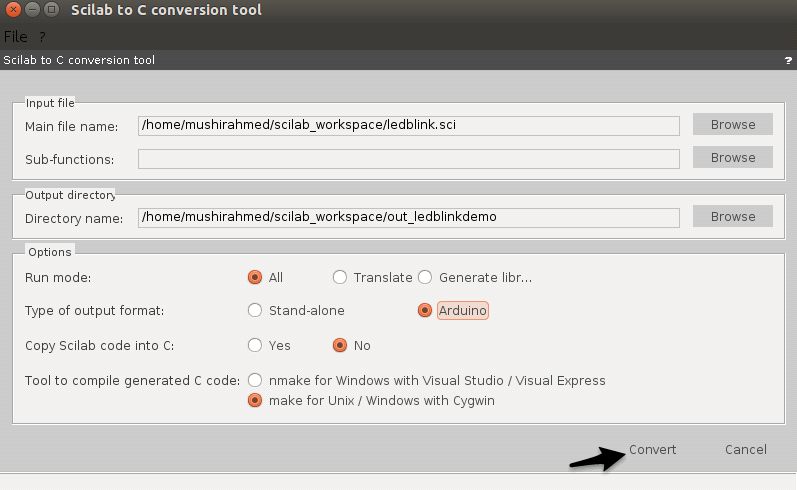
\includegraphics[scale=0.4]{img/gui_convert_btn}
   \caption {\small{Select output folder}}
   \label{fig:convert}
  }
  \end{figure}

  \item After clicking `Convert', scilab code will be run in scilab, to check for any errors. If code runs successfully, a prompt will occur asking if you 
  want to continue to code conversion or not. Select `Yes'. If scilab code doesn’t run correctly then code conversion is stopped there itself. 
  Correct the scilab code and follow the steps again.
  \item After selecting `Yes' for code conversion, code conversion starts. If code conversion is done successfully, you will see the message in command window.
  \item Generated code can be seen in output folder. By default a makefile is generated which uses `GCC' compiler to compile the C code. 
  You can compile this code using `make'. Open output folder in terminal and type `make' and press Enter. Once code is compiled successfully, it is run in terminal 
  and output can be seen in terminal window. Check the output for correctness. If code did not behave as expected, correct the scilab code and follow the process again.

 \end{enumerate}

  \item \textbf{Generating code for Arduino}
  \begin{enumerate}
  \item Write the scilab script first which is to be converted to C. Scilab code can contain single file or many files, but each file must be a scilab function. 
  There must be one main scilab file in case project contains many files, from which execution of code starts. All scilab files must be in a single folder. You can verify
  working of scilab script by runnig it on an Arduino board. Modify the script untill code behaves as expected. Once script is finalised, remove the commands 
  `open\_serial' 
  and `close\_serial'.
  
  \item Type `sci2c\_gui' or `scilab2c' in scilab console. This will prompt the GUI of Scilab2C extension as shown in figure  \ref{fig:gui}
  
  \item Click `Browse' next to `Main file name' textbox, browse to location of main scilab file and select it. (Refer figure \ref{fig:main})
  \item If scilab code contains many files, select folder containing these file by clicking `Browse' next to `Sub-functions' textbox.
  
  \item Create a new folder somewhere on the disk, preferably in same folder containing scilab files. Select this newly created folder by clicking 
  `Browse' next to `Directory name' textbox. (Refer figure \ref{fig:output})
  \item Choose appropriate options from `Options' box. Different options are explained below:
  \begin{enumerate}
   \item Run mode : If only directory structure is to generated in output directory, select `Generate library'. If only conversion of scilab files is to be done, select
   `Translate'. In case both are to be done, select `All'. 
   \item Target platform : To generate C code for arduino, select `Arduino' from dropdown. (Refer figure \ref{fig:arduino})
    \begin{figure}
    \centering
    {
    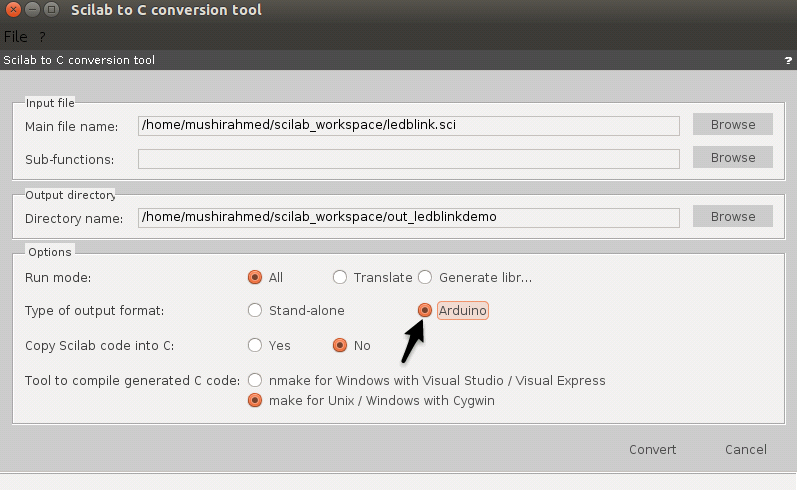
\includegraphics[scale=0.4]{img/gui_arduino}
    \caption {\small{Select `Standalone C' from dropdown}}
    \label{fig:arduino}
    }
    \end{figure}

   \item Copy scilab code into C: Select `Yes' or `No' accordingly.
   \item Tool to complie generated C code: Select appropriate option depending upon platform on which generated code will be complied. 
  \end{enumerate}
  \item Confirm everything again and then press `Convert’ button. (Refer figure \ref{fig:convert})
  \item Code conversion will start, promting different messages in command window. If conversion completes successfully, prompt will occur in command window indicationg the
  same.
  \item Generated code can be seen in output folder. A separate folder named `Arduino' is created, which contains a makefile and an arduino sketch file $-$ sci2c\_arduino.ino.
  \item Open `Makefile' using suitable text editor. Change following parameters according to board and connection:
  \begin{enumerate}
   \item  BOARD\textunderscore TAG
   \item ARDUINO\textunderscore PORT
  \end{enumerate}
  \item Open the terminal and change current directory to the directory containing modified Arduino sketch and then compile by typing `make' in terminal.
  \item If code is compiled successfully, you can upload it to arduino using `make upload' command.
  \item If code doesnot behave as expected, modify sclab code and follow the steps again.

 \end{enumerate}
 \item Generating code for AVR
\end{itemize}





\end{document}